
\documentclass[
   ngerman          % neue deutsche Rechtschreibung
  ,a4paper          % Papiergrösse
  ,twoside          % Zweiseitiger Druck (rechts/links)
  ,12pt             % Schriftgrösse
%  ,pdftex
%  ,disable         % Todo-Markierungen auschalten
]{report}

\usepackage[utf8]{inputenc}

\usepackage[table]{xcolor} % Must be before usapackage{bericht}, because clashing package
\usepackage{varioref}

\usepackage{bericht}
\usepackage{listingsutf8}

\lstdefinelanguage{Java}{
  showspaces=false,
  showtabs=false,
  breaklines=true,
  showstringspaces=false,
  breakatwhitespace=true,
  commentstyle=\color{pgreen},
  keywordstyle=\color{pblue},
  stringstyle=\color{pred},
%  basicstyle=\fontsize{9}{11}\ttfamily,
  moredelim=[il][\textcolor{pgrey}]{$.$},
  moredelim=[is][\textcolor{pgrey}]{\%\%}{\%\%},
  frame=single,
  tabsize=2,
  keywords={private, INDArray, double, int, new, for, return, Vector3}
}

\lstdefinelanguage{prepro}{
  showspaces=false,
  showtabs=false,
  breaklines=true,
  showstringspaces=false,
  breakatwhitespace=true,
  commentstyle=\color{pgreen},
  keywordstyle=\color{pblue},
  stringstyle=\color{pred},
%  basicstyle=\fontsize{9}{11}\ttfamily,
  moredelim=[il][\textcolor{pgrey}]{$.$},
  moredelim=[is][\textcolor{pgrey}]{\%\%}{\%\%},
  frame=single,
  tabsize=2,
  keywords={function, returns, import, export, vec3, mat}
}

\lstdefinelanguage{docker}{
	numbers=left,
	keywords={FROM, RUN, COPY, ADD, ENTRYPOINT, CMD,  ENV, WORKDIR, EXPOSE, LABEL, USER, VOLUME, STOPSIGNAL, ONBUILD, MAINTAINER},
	keywordstyle=\color{blue}\bfseries,
	identifierstyle=\color{black},
	sensitive=false,
	comment=[l]{\#},
	commentstyle=\color{purple}\ttfamily,
	stringstyle=\color{red}\ttfamily,
	morestring=[b]',
	morestring=[b]",
	breaklines=true
}

\lstdefinelanguage{bash}{
	numbers=left,
	keywords={if, then, else, fi, while, do, done, sleep, service, cd, rm, touch, apt, apt-get, echo, docker},
	keywordstyle=\color{blue}\bfseries,
	identifierstyle=\color{black},
	sensitive=false,
	comment=[l]{\#},
	commentstyle=\color{purple}\ttfamily,
	stringstyle=\color{red}\ttfamily,
	morestring=[b]',
	morestring=[b]",
	breaklines=true
}

%\lstdefinelanguage{bash}{
%		basicstyle=\ttfamily,
%		numbers=left,
%		showstringspaces=false,
%		commentstyle=\color{purple},
%		keywordstyle=\color{blue},
%		inputencoding=utf8,
%		extendedchars=true
%	basicstyle=\ttfamily,
%	numbers=left,
%	showstringspaces=false,
%	inputencoding=utf8,
%	extendedchars=true,
%	keywords={FROM, RUN, COPY, ADD, ENTRYPOINT, CMD,  ENV, WORKDIR, EXPOSE, LABEL, USER, VOLUME, STOPSIGNAL, ONBUILD, MAINTAINER},
%	keywordstyle=\color{blue}\bfseries,
%	identifierstyle=\color{black},
%	sensitive=false,
%	comment=[l]{\#},
%	commentstyle=\color{purple}\ttfamily,
%	stringstyle=\color{red}\ttfamily,
%	morestring=[b]',
%	morestring=[b]"
%}

%\lstdefinelanguage{docker-compose}{
%	keywords={image, environment, ports, container_name, ports, volumes, links},
%	keywordstyle=\color{blue}\bfseries,
%	identifierstyle=\color{black},
%	sensitive=false,
%	comment=[l]{\#},
%	commentstyle=\color{purple}\ttfamily,
%	stringstyle=\color{red}\ttfamily,
%	morestring=[b]',
%	morestring=[b]"
%}
\lstdefinelanguage{docker-compose-2}{
	keywords={version, volumes, services},
	keywordstyle=\color{blue}\bfseries,
	keywords=[2]{image, environment, ports, container_name, ports, links, build, hostname, networks, deploy},
	keywordstyle=[2]\color{purple}\bfseries,
	identifierstyle=\color{black},
	sensitive=false,
	comment=[l]{\#},
	commentstyle=\color{purple}\ttfamily,
	stringstyle=\color{red}\ttfamily,
	morestring=[b]',
	morestring=[b]"
}

\lstset{
	basicstyle=\ttfamily,
	showstringspaces=false,
	commentstyle=\color{purple},
	keywordstyle=\color{blue},
	inputencoding=utf8,
	extendedchars=true
}

% Hurenkinder und Schusterjungen verhindern
\clubpenalty = 10000
\widowpenalty = 10000
\displaywidowpenalty = 10000

\usepackage[toc, style=altlist, nonumberlist, xindy]{glossaries}
\defglsdisplayfirst[main]{#1#4\protect\footnote{#2}} %Fussnote bei erster Verwendung von GLS entry


\newglossaryentry{Inhalt}{
	name={Inhalt},
	description={Daten, welche auf den \glspl{Portal-Homepage} angezeigt werden, z.B. Lottodaten, Wetterdaten, Bundesliga-Liveticker und das Horoskop},
	plural={Inhalte}
}

\newglossaryentry{Portal-Homepage}{
	name={Portal-Homepage},
	description={Die Startseite einer der Portale web.de, gmx.net, gmx.ch, gmx.at und home.1und1.de},
	plural={Portal-Homepages}
}

\makeglossaries

%%%%%%%%%%%%%%%%%%%%%%%%%%%%%%%%%%%%%%%%%%%%%%%%%%%%%%%%%%%%%%%%%%%%%%%%%%%%%%%
%% Angaben zur Arbeit
%%%%%%%%%%%%%%%%%%%%%%%%%%%%%%%%%%%%%%%%%%%%%%%%%%%%%%%%%%%%%%%%%%%%%%%%%%%%%%%

\newcommand{\Autor}{Sebastian Bernauer}
\newcommand{\MatrikelNummer}{7390071}
\newcommand{\Kursbezeichnung}{TINF16B5}

\newcommand{\FirmenName}{United Internet AG}
\newcommand{\FirmenStadt}{Karlsruhe}
\newcommand{\FirmenLogoDeckblatt}{}

\newcommand{\BetreuerFirma}{Max Mustermann}
\newcommand{\BetreuerDHBW}{TODO: Rausfinden}

\newcommand{\Was}{Studienarbeit}

%%%%%%%%%%%%%%%%%%%%%%%%%%%%%%%%%%%%%%%%%%%%%%%%%%%%%%%%%%%%%%%%%%%%%%%%%%%%%%%%%%%%%

\newcommand{\Titel}{Entwicklung einer DSL zum Rechnen mit mathematischen Formeln für Anwendungen im Maschinellem Lernen}
\newcommand{\AbgabeDatum}{XX.XX.20XX}
\newcommand{\Dauer}{XX Wochen}
\newcommand{\Abschluss}{Bachelor of Science}
\newcommand{\Studiengang}{Angewandte Informatik}

\hypersetup{%%
  pdfauthor={\Autor},
  pdftitle={\Titel},
  pdfsubject={\Was}
}

\bibliography{bericht}

%%%%%%%%%%%%%%%%%%%%%%%%%%%%%%%%%%%%%%%%%%%%%%%%%%%%%%%%%%%%%%%%%%%%%%%%%%%%%%%

\begin{document}

{
	\setstretch{1.0}
	
\begin{titlepage}
	\begin{center}
		\vspace*{-2.2cm}
		\FirmenLogoDeckblatt\hfill
\includegraphics[width=4cm]{logos/DHBW}\\[2cm]
		{\Huge \Titel}\\[1.4cm]
		{\Huge\scshape \Was}\\[1.4cm]
		{\large für die Prüfung zum}\\[0.5cm]
		{\Large \Abschluss}\\[0.5cm]
		{\large des Studienganges \Studiengang}\\[0.5cm]
		{\large an der}\\[0.5cm]
		{\large Dualen Hochschule Baden-Württemberg Karlsruhe}\\[0.5cm]
		{\large von}\\[0.5cm]
		{\large\bfseries \Autor}\\[0.5cm]
		{\large Abgabedatum \AbgabeDatum}
		\vfill
	\end{center}
	\begin{tabular}{l@{\hspace{2cm}}l}
		Bearbeitungszeitraum	         & \Dauer 			\\
		Matrikelnummer	                 & \MatrikelNummer		\\
		Kurs			         & \Kursbezeichnung		\\
		Ausbildungsfirma	         & \FirmenName			\\
		& \FirmenStadt			\\
		Betreuer & Oliver Rettig		\\
		%& Marcus Strand \\ % Temporär
		%Gutachter der Studienakademie	 & \BetreuerDHBW		\\
	\end{tabular}
\end{titlepage}

}

%%%%%%%%%%%%%%%%%%%%%%%%%%%%%%%%%%%%%%%%%%%%%%%%%%%%%%%%%%%%%%%%%%%%%%%%%%%%%%%

% Nur für Bachelorarbeiten einfügen:

\newpage
\thispagestyle{empty}
\begin{framed}
\begin{center}
\Large\bfseries Erklärung
\end{center}
\medskip
\noindent
Ich versichere hiermit, dass ich meine \Was\ mit
dem Thema: \enquote{\Titel} selbstständig verfasst und keine anderen als die angegebenen Quellen und
Hilfsmittel benutzt habe. Ich versichere zudem, dass die eingereichte elektronische Fassung mit der
gedruckten Fassung übereinstimmt.

\vspace{1cm}
\noindent
\underline{\hspace{4.5cm}}\hfill\underline{\hspace{6.15cm}}\\
Ort~~~~~~~~~~Datum\hfill Unterschrift\hspace{4cm}
\end{framed}

%\vfill
%%Sofern von der Ausbildungsstätte ein Sperrvermerk gewünscht wird, ist folgende Formulierung zu verwenden:
%\begin{framed}
%\begin{center}
%\Large\bfseries Sperrvermerk
%\end{center}
%\medskip
%\noindent
%Der Inhalt dieser Arbeit darf weder als Ganzes noch in Auszügen Personen
%außerhalb des Prüfungsprozesses und des Evaluationsverfahrens zugänglich gemacht
%werden, sofern keine anders lautende Genehmigung der Ausbildungsstätte vorliegt.
%\end{framed}

%%%%%%%%%%%%%%%%%%%%%%%%%%%%%%%%%%%%%%%%%%%%%%%%%%%%%%%%%%%%%%%%%%%%%%%%%%%%%%%
\endinput
%%%%%%%%%%%%%%%%%%%%%%%%%%%%%%%%%%%%%%%%%%%%%%%%%%%%%%%%%%%%%%%%%%%%%%%%%%%%%%%


%%%%%%%%%%%%%%%%%%%%%%%%%%%%%%%%%%%%%%%%%%%%%%%%%%%%%%%%%%%%%%%%%%%%%%%%%%%%%%%

\begin{abstract}
TODO
\end{abstract}

\newpage
{
	\setstretch{1.1}
	\tableofcontents           % Inhaltsverzeichnis hier ausgeben
}


\chapter{Motivation}
Immer öfter werden Probleme der realen Welt mittels neuronaler Netze gelöst.
Allerdings kann man in den meisten Fällen nicht einfach das neuronale Netz auf die gemessenen Daten angewendet werden.
Die Daten müssen vorher aufbereitet werden und gegebenenfalls unwichtige Daten entfernt werden.
Dies geschieht mittels verschiedener Frameworks in verschiedenen Sprachen.
Es soll eine \ac{DSL} entwickelt werden, die genau auf diesen Anwendungsfall zugeschnitten ist.
Durch die \ac{DSL} soll einen einheitliche Sprache geschaffen werden, welche das Vorprozessieren der Daten vereinfacht.
Die Sprache soll plattformübergreifend sein und \ac{CPU}- und \ac{GPU}-Berechnungen ermöglichen.

%%%%%%%%%%%%%%%%%%%%%%%%%%%%%%%%%%%%%%%%%%%%%%%%%%%%%%%%%%%%%%%%%%%%%%%%%%%%%%%
\endinput
%%%%%%%%%%%%%%%%%%%%%%%%%%%%%%%%%%%%%%%%%%%%%%%%%%%%%%%%%%%%%%%%%%%%%%%%%%%%%%%


\chapter{Überblick über Technologien}

Das Aufbereiten der Daten für das neuronale Netz kann in mehreren Frameworks in mehreren Sprachen erfolgen.
Oft wird für das Vorverarbeiten die gleiche Sprache wie für das neuronale Netz verwendet.
Die gängigsten Frameworks sind in \tab{tab:Frameworks} gelistet.

\begin{table}[H]
	\centering
	\begin{tabular}{ | p{3cm} | p{3cm} | }
		\hline \rowcolor{gray!15}
		\textbf{Framework} & \textbf{Sprache} \\ \hhline{|=|=|}
		Tensorflow & Python \\ \hline
		DL4J & Java \\ \hline
	\end{tabular}
	\caption{Die gängigsten Frameworks für maschinelles Lernen}
	\label{tab:Frameworks}
\end{table}

\section{Unterschied Compiler, Transpiler und Interpreter}
\begin{description}
	\item{\textbf{Compiler}}\newline{Übersetzt von einer höheren Sprache in eine niedrigere Sprache.}
	\item{\textbf{Transpiler}}\newline{Übersetzt zwischen zwei Sprachen mit ungefähr gleichem Abstraktionsgrad.}
	\item{\textbf{Interpreter}}\newline{Führt Code einer höheren Sprache direkt aus ohne den Code in eine andere Sprache zu übersetzen.}
\end{description}

\section{ND4J}
ND4J ist eine Framework für die Sprache Java, in welchem effiziente Matrizenoperationen durchgeführt werden können.
Es kann auf der \ac{CPU} oder \ac{GPU} ausgeführt werden.
In ND4J ist größtenteils nur das Konstrukt einer Matrix bekannt, Vektoren oder Skalare sind nur ein Spezialfall einer Matrix.

%%%%%%%%%%%%%%%%%%%%%%%%%%%%%%%%%%%%%%%%%%%%%%%%%%%%%%%%%%%%%%%%%%%%%%%%%%%%%%%
\endinput
%%%%%%%%%%%%%%%%%%%%%%%%%%%%%%%%%%%%%%%%%%%%%%%%%%%%%%%%%%%%%%%%%%%%%%%%%%%%%%%

\chapter{Aufgabenstellung}
\section{Zu Grunde liegendes Framework}
Im RaHM-Lab hat sich der Einsatz von dem Framework ND4J in der Programmiersprache Java für den Praxiseinsatz bewährt.
Daher soll die in dieser Arbeit entwickelte \ac{DSL} auf diesem Framework aufbauen.

\section{Compiler und Interpreter}
Die zu entwickelnde DSL soll dem Vorprozessieren von Daten für die Anwendung von maschinellen Lern-Methoden dienen.
Für die \ac{DSL} kommt ein Compiler oder Interpreter in Frage.
Ein Transpiler ist nicht möglich, da es keine in der Praxis verwendete Sprache für das Vorprozessieren der Daten gibt, in die übersetzt werden kann.
In der \tab{tab:Vorteile_Compiler_Interpreter} werden die Implementierungsmöglichkeiten mittels Compiler und Interpreter gegenüber gestellt.\\
Wegen der Vorteile (vornehmlich das Debugging) von Interpretern im Vergleich zu Compiler soll PrePro als Interpreter implementiert werden.

\begin{table}[H]
	\centering
	\begin{tabular}{ | p{3cm} | p{6cm} | p{6cm} | }
		\hline \rowcolor{gray!15}
		\textbf{Implemen-tierung} & \textbf{Vorteile} & \textbf{Nachteile} \\ \hhline{|=|=|=|}
		Compiler & Generierter Java-Code kann auf jeder \ac{JVM} ausgeführt werden, es wird kein Interpreter benötigt. & Debugging ist nur in dem generierten Java-Code möglich. \\ \hline
		Interpreter & Debugging leichter möglich & Möglicherweise nicht so performant \\ \hline
	\end{tabular}
	\caption{Vor- und Nachteile einer Implementierung mittels Compiler oder Interpreter}
	\label{tab:Vorteile_Compiler_Interpreter}
\end{table}

\label{sec:usedTechnologies}
\section{Verwendete Technologien}
Die \ac{DSL} wird mittels einem Interpreter ausgeführt.
Dieser ist in Java (genauer: Groovy) geschrieben und baut auf folgenden Technologien auf:
\begin{description}
	\item{\textbf{ND4J}}\newline Matrizen-Berechnungen werden mittels dem ND4J-Framework durchgeführt.
	\item{\textbf{Java}}\newline Das ND4J-Framework ist in der Programmiersprache Java verfügbar. Damit der Interpreter es verwenden kann, wird in dieser Sprache geschrieben.
	\item{\textbf{Groovy}}\newline Groovy ist eine Sprache, die auf Java aufbaut und kompatibel ist. Sie unterstützt zum Beispiel dynamic dispatching\footnote{\url{https://en.wikipedia.org/wiki/Dynamic_dispatch}}.
	\item{\textbf{Antlr}}\newline Antlr in der Version 4 wird für das Parser der eingegebenen Programme verwendet. Für das Netbeans-Plugin wird Antlr in der Version 3 verwendet.
\end{description}

%%%%%%%%%%%%%%%%%%%%%%%%%%%%%%%%%%%%%%%%%%%%%%%%%%%%%%%%%%%%%%%%%%%%%%%%%%%%%%%
\endinput
%%%%%%%%%%%%%%%%%%%%%%%%%%%%%%%%%%%%%%%%%%%%%%%%%%%%%%%%%%%%%%%%%%%%%%%%%%%%%%%


\chapter{Design der DSL}

\section{Funktionen}
In Programmiersprachen werden meist manche Codezeilen häufig benötigt.
Anstatt diese Zeilen mehrfach zu kopieren, kann man diese Zeilen in eine sogenannte Funktion packen.
Diese Funktionen können an beliebiger Stelle im Code aufgerufen werden.
Auf diese Weise kann der entstandene Code gekürzt werden.
Dies erhöht die Lesbarkeit und verhindert Kopierfehler.\\
Daher soll die zu entwickelnde \ac{DSL} auch Funktionen unterstützen.\\
\textbf{Parameter}\\
Funktionen können auch parametrisiert werden, was bedeutet, dass bei dem Aufruf der Funktion Werte mitgegeben werden können.
Jede Funktion hat ihren eigenen Variablen-Gültigkeitsbereich, das bedeutet, dass Funktionen ihren Variablen den gleichen Namen geben können, aber unterschiedliche Variablen verwenden.
Wenn eine Funktion Werte übergeben bekommen möchte, so muss sie diese mitsamt ihrem Typ angeben.\\
\textbf{Rückgabetyp}\\
Funktionen können eine Wert zurückgeben.
Dieser muss einen bestimmten Typ haben.
In der DSL ist ein Rückgabetyp möglich und muss mittels ``returns <Typ>'' gekennzeichnet sein.
Ist keine Angabe gemacht ist keine Rückgabe vorhanden.\\
\textbf{Überladen von Funktionen}\\
Eine Funktion bezeichnet man als überladen, wenn es mehrere Funktionen mit gleichen Namen, aber unterschiedlicher Zahl oder Art von Parametern gibt.
In der DSL ist ein Überladen von Funktionen nicht vorgesehen, könnte aber nachträglich noch implementiert werden.\\
Ein Beispiel von verschiedenen Funktionen befindet sich in \code{lst:Bsp_Funktionen}.\\

\subsection{Main-Funktion in der \acs{DSL}}
Jedes prozedurale Programm benötigt einen Einstiegspunkt, wo das Programm gestartet wird.
Da die DSL ein Framework verwendet, welches in Java geschrieben ist, ist es nicht unwahrscheinlich, dass die zukünftigen Nutzer vorher in Java programmiert haben.
Daher wurde als Einstiegspunkt des Programms - wie in Java - eine Main-Funktion gewählt.
In der DSL besitzt sie keine Parameter.
Um Daten in sein Programm zu laden wurde der Ansatz eines DataSets gewählt, mehr dazu in \kap{sec:Import}.

\subsection{Weglassen der Main-Funktion}
Es gibt mehrere Gründe, warum die Definition einer Main-Funktion unnötig ist:
\begin{itemize}
\item Es gibt Anwendungsfälle in denen ein verkürzte Syntax wünschenswert ist, und auf die Main-Funktion verzichtet werden kann.
\item Kompatibilität mit bisher bestehenden anderen Tools, die keine Funktionen bieten, sondern nur eine Liste von Anweisungen entgegennehmen.
\end{itemize}
Deshalb wurde die Main-Funktion in \acs{PrePro} optional implementiert und muss nicht deklariert werden.
Es reicht aus die Befehle untereinander zu schreiben.\\
Trotzdem wird es als guter Stil erachtet, eine Main-Funktion zu deklarieren.

\begin{lstlisting}[language=prepro, label={lst:Bsp_Funktionen}, caption={Beispiel Funktionen}, captionpos=b]
function main() {
	import vec3 p1, vec3 p2, vec3 p3;

	vec3 x = calculateDifference(p1, p2);
	vec3 s = calculateDifference(p1, p3);
	vec3 y = s X x;
	vec3 z = y X x;


	printResults(x, y, z);

	export x, y, z;
}

function calculateDifference(vec3 p1, vec3 p2) returns vec3 {
	return p2 - p1;
}

function printResults(vec3 x, vec3 y, vec3 z) {
	print x;
	print y;
	print z;
}
\end{lstlisting}

\section{Variablen}
Die \ac{DSL} ist für den Einsatz auf Zeitreihenberechnungen ausgelegt.
Daher stellt in der \ac{DSL} jede Variable eine Zeitreihe dar.
Die Operationen der \ac{DSL} sind immer auf Zeitreihen definiert.\\
Beispielsweise der Ausdruck \texttt{x = a - b;}:
In diesem Fall sind \texttt{a} und \texttt{b} Zeitreihen von Sensordaten.
Die Variable \texttt{x} repräsentiert eine neue Zeitreihe, die durch elementweise Subtraktion jedes Zeitelements entstanden ist.\\
Der Vorteil liegt darin, dass der simple Ausdruck \texttt{x = a - b;} sehr leicht les- und wartbar ist.
Wenn jede Variable keine Zeitreihe, sondern ein einzelner Messpunkt wäre, müsste man eine Schleife verwenden oder sich eigene Methoden definieren bzw. (falls in der Sprache möglich) die Operatoren überschreiben.\\
Variablen haben in der \ac{DSL} immer einen Typ.
Bei dem Anlegen einer Variablen muss dieser auch immer definiert werden.
Ein Typ ist zum Beispiel ein Vector3 (vec3) oder eine Matrix (mat).
Ein Vector3 ist eine Zeitreihe von Vektoren mit der Länge 3, eine Matrix eine Zeitreihe von Matrizen.
Ein dem Programm zur Verfügung gestellter Vektor der Länge 3 kann nun als Vector3 oder auch als Matrix aufgefasst werden.
Daher muss dem Interpreter beim Anlegen der Variablen immer der Typ mitgeteilt werden.
Wenn die Variable schon existiert, muss der Typ nicht erneut angegeben werden.\\
Ein Beispiel befindet sich in \code{lst:Bsp_Variablenzuweisung}.\\
Das Import-Statement wird in \kap{sec:Import} erläutert, relevant ist an dieser Stelle nur, dass mit dem Import Daten aus einem DataSet geladen werden.

\begin{lstlisting}[language=prepro, label={lst:Bsp_Variablenzuweisung}, caption={Beispiel Variablenzuweisung}, captionpos=b]
import vec3 p1, vec3 p2, vec3 p3;

vec3 x = p2 - p1;
vec3 s = p3 - p1;
vec3 y = s X x;
vec3 z = y X x;
\end{lstlisting}

\section{DataSet}
Ein DataSet ist in der \ac{DSL} eine Sammlung von Variablen.
In das DataSet können beliebig viele Zeitreihen und Konstanten unter einem Namen gespeichert werden.
Es ist nicht möglich zwei Elemente mit dem gleichen Namen abzulegen.
Eine Variable kann mittels der Funktion \texttt{INDArray getVariable(String variableName)} aus dem DataSet ausgelesen werden.

\section{Import \& Export}
\label{sec:Import}

Ein Programm, das nur Berechnungen anstellt, ohne ein Ergebnis zu liefern, erscheint auf den ersten Blick unnötig.
Es muss die Möglichkeit haben, Daten zu lesen und zu schreiben.
Im Falle der DSL wird ein eigenes DataSet definiert.
Das Programm erhält bei der Ausführung ein DataSet als Eingabe und gibt als Ausgabe ein DataSet zurück.
In das Eingabe-DataSet werden alle Variablen gespeichert, die für die Berechnungen benötigt werden.
In dem Ausgabe-DataSet sind anschließend alle Variablen gespeichert, die berechnet wurden.\\
Die Verwendung eines DataSet hat gegenüber dem Übergeben mittels Parametern in die Main-Funktion folgende Vorteile:
\begin{itemize}
\item Es gibt nur einen Rückgabetyp (DataSet).
Andernfalls müsste ein Konstrukt ersonnen werden, mehrere Objekte (z.B. Zeitreihen oder Konstanten) von der Main-Funktion zurückgeben zu lassen.
\item Einfacher Aufruf der Main-Funktionen (ab 4 Parametern wird der Funktionsaufruf unübersichtlich\cite{parameterCount}). Statt 20 Parameter zu übergeben kann übersichtlich das DataSet zusammengebaut werden und als einziges Argument übergeben werden.
\item Einfaches ``Weiterreichen'' von DataSets zwischen mehreren PrePro-Programmen.
Falls mehrere PrePro-Programme nacheinander ausgeführt werden, kann das Ausgabe-DataSet des ersten Programms als Eingabe-DataSet des zweiten Programms genommen werden.
\end{itemize}

\subsection{Optionale Imports}
Es soll möglich sein, Importe in die Main-Funktion als optional zu kennzeichnen.
Diese werden mit dem Schlüsselwort \texttt{optional} gekennzeichnet.
Eine Beispiel mit optionalen Imports ist in \code{lst:OptionalImport} gegeben.
Wenn die angegebene, zu importierende Variable nicht in dem DataSet existiert, wird keine Fehlermeldung erzeugt, sondern die Variable nicht importiert.\\
\textbf{Achtung}: Wenn ein Import optional ist und die Variable nicht in dem DataSet existierte, wurde die Variable nicht geladen.
Wenn nun in dem Programm versucht wird auf die Variable zuzugreifen wird eine Fehlermeldung erzeugt, dass die Variable nicht definiert sei.
Deshalb ist es wichtig, die Gültigkeit der Variablen mittels der \texttt{exists}-Funktion zu prüfen, die im nächsten Kapitel vorgestellt wird.
Wenn bei der Konstruktion des Ausführungspfad nicht aufgepasst wird, kann auf eine nicht existierende Variable zugegriffen werden.
Das ist vergleichbar mit Nullpointern, die in eine Funktion hereingegeben werden können und zunächst mal auf \texttt{!= null} geprüft werden müssen.\\
Deshalb ist es definitiv nicht ratsam, alle Imports als optional zu kennzeichnen.
Vielmehr sollten nur die wirklich optionalen Variablen als optional gekennzeichnet werden.

\begin{lstlisting}[language=prepro, label={lst:OptionalImport}, caption={PrePro-Code mit optionalen Imports}, captionpos=b]
function main() {
	import vec3 p1, optional const quaternion_1, optional mat4 notPresent;

	const isPresent = exists(p1);
	const isNotPresent = foo();

	export p1, quaternion_1, isPresent, isNotPresent;
}

function foo() returns const {
	return exists(notPresent);
}
\end{lstlisting}

\subsection{Die exists-Funktion}
Mittels der Funktion \texttt{exists(<VariablenName>)} kann abgefragt werden, ob diese Variable geladen wurde.
Wurde die Variable zur Verfügung gestellt, gibt die Funktion eine 1 zurück, andernfalls eine 0.
Nach Abschluss der Berechnungen in \code{lst:OptionalImport} hat die Variable \texttt{isPresent} der Wert 1, die Variable \texttt{not Present} den Wert 0.
Dies ist in folgendem Fall nützlich:
In ein Programm werden zwei Koordinaten-Zeitreihen A und B gegeben.
Im Regelfall wird auf dem Mittelpunkt zwischen diesen Punkten gearbeitet.
Ist jedoch die Variable A nicht definiert, soll für die Berechnung B verwendet werden, und anders herum.
Eine kleine Abweichung wird hier in Kauf genommen.
Dieser Fall mag ungewöhnlich wirken, warum sollte der Code nicht einfach an die Verwendung von A oder B angepasst werden?
Dies gibt mehr Sinn, wenn ein Skript allgemein verwenden werden soll um häufig genutzte Berechnungen auszulagern.
In diesem Fall möchte man nicht jedes Mal die Berechnung aufs neue anpassen, sondern die Funktion einmal allgemein schreiben und die Ausführung abhängig von den gegebenen Daten machen.
Das oben genannte Beispiel mit A und B könnte in etwa so ausgedrückt werden.
Der Code in \code{lst:OptionalImportExample}, soll das Prinzip verdeutlichen.
\begin{lstlisting}[language=prepro, label={lst:OptionalImportExample}, caption={PrePro-Code mit optionalen Imports}, captionpos=b]
import optional vec3 a, optional vec3 b;

vec3 center = (exists(a) && exists(b)) ** (a + b) / 2
|| exists(a) ** a
|| exists(b) ** b
|| throw "Neither a or b exists";

export center;
\end{lstlisting}
Falls die Variable a und b beide existieren ergibt der Ausdruck \texttt{(exist(a) \&\& exist(b))} eine 1, andernfalls eine 0.
Wichtig ist an dieser Stelle, dass die Multiplikationen lazy sind:
Falls a existiert und b nicht, ergibt der Ausdruck \texttt{(exist(a) \&\& exist(b))} eine 0, der Interpreter rechnet dann weiter, also \texttt{* ( a + b ) / 2}.
Das Ergebnis einer Multiplikation ist immer null, soweit ist die Rechnung korrekt, da durch das \texttt{||} die anderen Fälle probiert werden.
Das Problem ist:
Der Interpreter versucht \texttt{* ( a + b ) / 2}. zu berechnen und erzeugt - vollkommen zurecht - eine Fehlermeldung, dass b nicht definiert ist.\\
Zur Lösung dieses Problems gab es 2 Möglichkeiten:
\begin{enumerate}
\item \textbf{Lazy Multiplikation}\\
Es wird ein neuer Multiplikations-Operator eingeführt, der den rechten Teil nur berechnet, wenn der linke Teil != 0 ist.
Dadurch würde nach dem Teil \texttt{(exist(a) \&\& exist(b))} die Berechnung abgebrochen, da der linke Teil 0 ergibt.
Durch das Abbrechen wird nicht versucht Variablen zu verwenden, die nicht definiert sind.
Für diesen neuen Multiplikations-Operator wurde ein neues Symbol definiert: ``**''.\\
\textbf{Vorteile}:
\begin{itemize}
\item Einfache Implementierung.
\item Wiederverwendung des Operators an anderer Stelle möglich.
\end{itemize}
\textbf{Nachteile}:
\begin{itemize}
\item Die Nutzer müssen einen zusätzlichen Operator kennen und verstehen.
\end{itemize}

\item \textbf{Dedizierte If-Statements}\\
In die \ac{DSL} PrePro wird noch das Konstrukt einer If-Verzweigung eingebaut.
Der beispielhafte PrePro-Code würde somit wie in \code{lst:OptionalImportExample_If} aussehen.
\begin{lstlisting}[language=prepro, label={lst:OptionalImportExample_If}, caption={PrePro-Code mit If-Statements und der exists-Funktion}, captionpos=b]
import optional vec3 a, optional vec3 b;

if(exists(a) && exists(b)) {
    vec3 center = ( a + b ) / 2;
} else if (exists(a)) {
    vec3 center = a;
} else if (exists(b)) {
    vec3 center = b;
}
<<OPTIONAL>>
else {
	throw "Neither a or b exists";
}
\end{lstlisting}
\textbf{Vorteile}:
\begin{itemize}
\item Leichter lesbar und verständlich.
\item Auch für andere Fälle als die Multiplikation ist das If-Statement verwendbar.
\end{itemize}
\textbf{Nachteile}:
\begin{itemize}
\item Erhöht die Anzahl der Codezeilen dramatisch.
\item Höherer Aufwand bei der Implementierung
\end{itemize}
\end{enumerate}
Aufgrund der einfacheren Implementierung und der kurzen, prägnanten Ausdrucksweise wurde die Variante der Lazy Multiplikation in PrePro umgesetzt.

\section{Kommentare}
In der \ac{DSL} wird einem Zeilen-Kommentar ein ``//'' vorangestellt.\\
Ein Block-Kommentar wird mit ``/*'' und ``*/'' umschlossen.

%%%%%%%%%%%%%%%%%%%%%%%%%%%%%%%%%%%%%%%%%%%%%%%%%%%%%%%%%%%%%%%%%%%%%%%%%%%%%%%
\endinput
%%%%%%%%%%%%%%%%%%%%%%%%%%%%%%%%%%%%%%%%%%%%%%%%%%%%%%%%%%%%%%%%%%%%%%%%%%%%%%%


\addtocontents{toc}{\protect\newpage}
\chapter{Implementierung der DSL}

\section{Lexer \& Parser}
Lexer und Parser werden beide von einer ANTLR4 Grammatik erzeugt.
Hierfür wird eine kombinierte Grammatik verwendet, die zugleich Lexer und Parser erzeugt.\\
Die Grammatik ist unter \texttt{src/main/java/de/sbernauer/prepro/parser} abgelegt.
Mittels dem Befehl \texttt{./generateLexerAndParser.sh} im Root-Verzeichnis des Projekts werden die benötigten Klassen von ANTLR aus der Grammatik generiert.
Dies ist notwendig, wenn Änderungen an der Grammatik durchgeführt wurden, damit diese in den Interpreter übernommen werden.

\section{Abstrakter Syntaxbaum}
Ein \ac{AST} ist ein Baum, der bei dem Parsen der Grammatik der \ac{DSL} aufgebaut wird.
Dieser wird anschließend von dem Interpreter abgearbeitet / ausgeführt.\\
Der Baum besteht aus Knoten, die in einer Baumstruktur an einer Wurzel hängen.
Jeder Knoten besitzt wiederum eine beliebige Anzahl an Kindknoten, diese kann auch 0 sein.
Es gibt einen einzigen Wurzelknoten, an dem der gesamte \ac{AST} aufgehängt ist.\\
In \abb{fig:AST_Example} ist ein beispielhafter \ac{AST} abgebildet.
Es ist ersichtlich, dass ein \ac{AST} schnell unübersichtlich wird.
Der in \abb{fig:AST_Example} abgebildete \ac{AST} wurde aus dem PrePro-Code in \code{lst:AST_Example} erzeugt.
Trotz, dass der ursprüngliche Sourcecode überschaubar ist, ist der entstandene \ac{AST} fast nicht mehr lesbar.
Dementsprechend groß werden die \acp{AST} bei längeren Programmen.
Da die \acp{AST} allerdings von dem Parser aufgebaut und von dem Interpreter abgearbeitet werden bekommt der Nutzer diese nie zu Gesicht.
\begin{figure}[H]
	\centering
	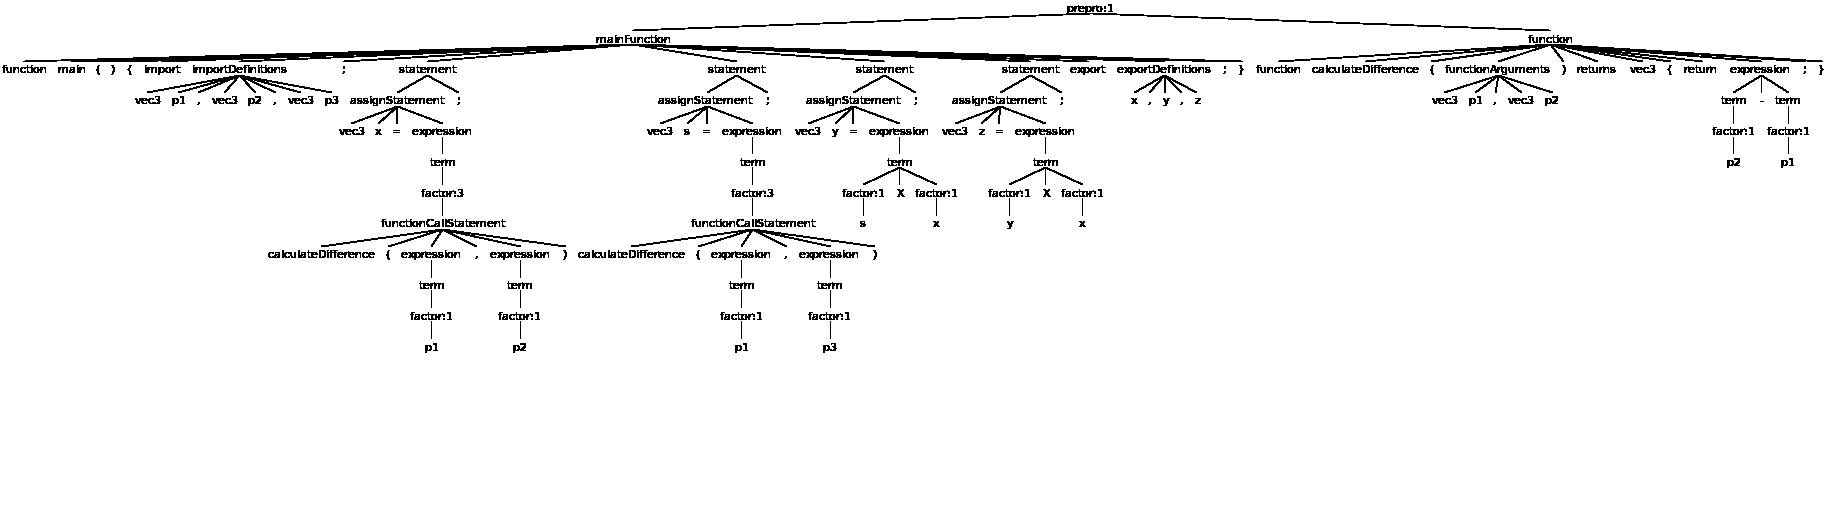
\includegraphics[width=\textwidth]{figures/parseTree}
	\caption{Beispielhafter \ac{AST}}
	\label{fig:AST_Example}
\end{figure}

\begin{lstlisting}[language=prepro, label={lst:AST_Example}, caption={PrePro-Code für den beispielhaften AST}, captionpos=b]
function main() {
    import vec3 p1;

    vec3 result = double(p1);
    result = result - p1;
    result = result - p1;

    export result;
}

function double(vec3 vec) returns vec3 {
    return add(vec, vec);
}

function add(vec3 a, vec3 b) returns vec3 {
    return a + b;
}
\end{lstlisting}
Ein \ac{AST}-Baum besteht nicht aus lauter gleichen Knoten, sondern aus vielen verschiedenen Klassen.
In PrePro gibt es eine Vielzahl an verschiedener Knoten-Typen, welche durch Java-Klassen repräsentiert werden.
Die Klassenhierarchie ist in \abb{fig:NodesHierachy} abgebildet.\\
Die dort aufgeführten Packages werden in den nachfolgenden Kapiteln im Detail erläutert.

\begin{figure}[H]
	\centering
	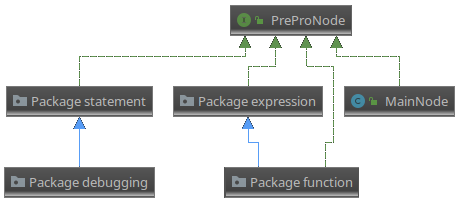
\includegraphics[width=\textwidth]{figures/uml_nodes}
	\caption{Die Knoten-Klassenhierarchie}
	\label{fig:NodesHierachy}
\end{figure}

\subsection{Wurzelknoten}
Die \texttt{MainNode} ist der Wurzelknoten des \ac{AST}.
Er beinhaltet als Kinder alle Funktionen, die in dem Programm definiert sind.
In Abbildung \abb{fig:AST_Example} sind die 3 Teilbäume ersichtlich, die den 3 Funktionen aus \code{lst:AST_Example} entsprechen.\\
Alle Knoten müssen das \texttt{PreProNode}-Interface implementieren.
Dieses ist ein leeres Interface, besitzt somit keine Funktionen und dient nur dazu, alle Knoten als Knoten zu markieren.

\subsection{Funktionen}
In PrePro gibt es Funktionen.
Direkt unter dem Wurzelknoten sind die Funktion-Knoten aufgehängt.
Sonst hängt nichts an dem Wurzelknoten.
Jede Funktion wird durch einen eigenen Knoten mitsamt Kindern dargestellt.
Zum Starten des Programms wird die Main-Funktion aus dem \ac{AST} herausgesucht und gestartet.
Eine Funktion hat Argumente, die ihr übergeben werden, diese müssen als Unterknoten in dem \ac{AST} gespeichert werden, damit sie bei der späteren Ausführung mit in die Funktion rein gegeben werden können.\\
Es wurde eine allgemeines \texttt{Function}-Interface definiert, welches die Funktionen \texttt{String getFunctionName()} und\\ \texttt{Variable execute(Arguments arguments, FunctionTable functionTable)} besitzt.\\
Das hat den Vorteil, dass das Interface unabhängig davon verwendet werden kann, ob die Funktion im Sourcecode definiert wurde oder von PrePro in Java-Code global zur Verfügung gestellt wurde.
Im ersteren Fall erzeugt der Parser eine \texttt{FunctionNode}, im zweiten Fall wird die Funktion in reinem Java spezifiziert.
Die \texttt{FuntionNode} führt die im Sourcecode angegebeben Statement-Nodes aus, die \texttt{CustomFunctionNode} ruft Java-Funktionen mittels Reflection auf.\\
Alle eben genannten Klassen sind im \texttt{nodes.function} Package abgelegt.

\subsection{Statements}
Eine Funktion besteht aus einer Reihe von Statements.
Eine Statement ist eine Anweisung, die ausgeführt wird und keine Rückgabe besitzt.
Dies grenzt sie von Expressions ab, die einen Wert zurückgeben.
Die Zeile \texttt{a = 1 + 2;} ist in ihrer Gesamtheit ein Statement, da es keine Rückgabe.\\
Als allgemeines Statement wurde die abstrakte Klasse \texttt{StatementNode} definiert.
Sie besitzt die Funktion\\ \texttt{void execute(SymbolTable symbolTable, FunctionTable functionTable)}
Alle Klassen, die von dieser Klasse erben, müssen die \texttt{execute}-Funktion implementieren.
Dazu zählt z.B. die \texttt{PrintStatementNode}, welche in der \texttt{execute}-Funktion einen Ausgabe auf dem Bildschirm erzeugen.

\subsection{Expression}
Die Teil \texttt{1 + 2} der Zeile \texttt{a = 1 + 2;} ist eine Expression.
Eine Expression ist ein (mathematischer) Ausdruck, der ausgeführt werden kann und einen Rückgabewert besitzt.
In einer Expression können neben mathematischen Operatoren, Konstanten, Variablen und Funktionsaufrufe beinhalten.
Die abstrakte Superklasse \texttt{ExpressionNode} definiert die Funktion\\
\texttt{Variable execute(SymbolTable symbolTable, FunctionTable functionTable)}.\\
Wichtig ist an dieser Stelle, dass die Funktion im Gegensatz zu der Funktion bei der \texttt{StatementNode} einen Wert vom allgemeinen Typ \texttt{Variable} zurück liefert.
Alle dafür nötigen Klassen sind in dem Package \texttt{nodes.expression} abgelegt.

\subsection{Debugging}
In PrePro ist zunächst eine rudimentäre Debugging-Möglichkeit eingebaut.
Es ist möglich an einer beliebigen Zeile im Code ein \texttt{break;} zu schrieben.
Bei der Ausführung stoppt der Interpreter in dieser Zeile und bietet eine kleine Kommandozeile um Variablen zu lesen und zu modifizieren.
Dieses Break-Statement ist ein Statement, erbt also von der \texttt{StatementNode}.
In der überschriebenen \texttt{execute}-Funktion wird auf die Eingabe und das Weiterspringen des Nutzers gewartet.

\section{Typsystem}
Das Typsystem von PrePro ist in \abb{fig:Typsystem} dargestellt.
Alle Variablen erben von er abstrakten Klasse \texttt{Variable}.
Es gibt die Untertypen \texttt{Vector}, \texttt{Marix}, \texttt{Scalar} und \texttt{Constant}.
Die Unterklassen \texttt{Vector} und \texttt{Matrix} haben wiederum Unterklassen für drei- und vierelementige Varianten.
Diese Unterklassen sind wichtig, da z.B. eine \texttt{Matrix3} mit einem \texttt{Vector3} multipliziert werden kann, allerdings nicht mit einem \texttt{Vector4}.\\
In der abstrakten Klasse \texttt{Variable} sind die Funktionen \texttt{add}, \texttt{sub}, \texttt{mul} und \texttt{div} definiert.
Werden die Funktionen auf der abstrakten Klasse aufgerufen, werfen sie eine Exception, dass die mathematische Operation nicht definiert sei.\\
Die Unterklassen haben nun die Möglichkeit, Operationen mit anderen Typen zu definieren.
Mittels Polymorphie und dynamic dispatching wird bei einer arithmetischen Operation die passende Funktion gesucht.
Falls keine passende Funktion wird die allgemeine - in der abstrakten Klasse definierte - Funktion verwendet, und daraufhin eine Exception geworfen, dass die mathematische Operation nicht definiert sei.

\begin{figure}[H]
	\centering
	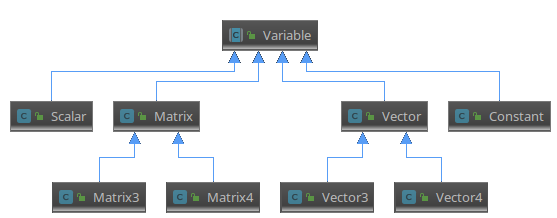
\includegraphics[width=\textwidth]{figures/typsystem}
	\caption{Typsystem von PrePro}
	\label{fig:Typsystem}
\end{figure}

\subsection{Darstellung der Typen in Java}
Alle Typen werden als \texttt{INDArray} von \texttt{ND4J} dargestellt.\\
Die Unterklassen besitzen einen Konstruktor, der ein \texttt{INDArray} übergeben bekommt.
In den Konstruktoren wird jeweils geprüft, ob die Dimensionen dem entsprechenden Typ entsprechen (z.B eine Matrix4 muss eine 4x4-Matrix übergeben bekommen).
Die einzige Ausnahme bildet der Typ ``Constant'', dieser bietet zusätzlich einen Konstruktur, dem ein \texttt{double} übergeben werden kann.
Intern wird aus dem \texttt{double} ein \texttt{INDArray} erzeugt.

\section{Implementierung der Operationen auf den Variablen-Typen}
In dem vorherigen Abschnitt wurden verschiedene Variablen-Typen herausgearbeitet.
Diese sind in \abb{fig:Typsystem} abgebildet.\\
Zwischen manchen der Typen sind Operationen, wie z.B. das Kreuzprodukt definiert.
Manche Typen können allerdings nicht sinnvoll kombiniert werden, z.B. eine Matrix3 und eine Matrix4.
Diese Operationen müssen in Java implementiert werden.
Ein erster Ansatz ist es, jedem Variablen-Typ die möglichen Operationen der Java-Klasse hinzuzufügen.
Dieser Ansatz wurde in dem \code{lst:Operationen_Matrix4} beispielsweise für die \texttt{Matrix4}-Klasse angewandt. Die Methoden sind jedoch lange nicht vollzählig.
\begin{lstlisting}[escapeinside={\%*}{*)},language=java, label={lst:Operationen_Matrix4}, caption={Implementierung der Operatoren in der Java-Klasse Matrix4}, captionpos=b]
%*
\begin{minted}[frame=single,framesep=10pt]{java}
public class Matrix4 {

	// same for sub, mul and div
	public Matrix4 add(Matrix4 right) {
		return new Matrix4(/* ... */);
	}

	// same for sub, mul and div
	public Matrix4 add(Constant right) {
		return new Matrix4(/* ... */);
	}

	// Cross-Product
	public Vector4 mul(Vector4 right) {
		return new Vector4(/* ... */);
	}
}
\end{minted}
\end{lstlisting}
Es ist zu erkennen, dass sehr viele Funktionen angelegt werden müssen.
Damit der Java-Compiler korrekt compilieren kann, müssen diese Funktionen in der Basisklasse \texttt{Variable} definiert werden und in den Unterklassen überschrieben werden.
Dies hat den Vorteil, dass in der Basis-Funktion in der Basis-Klasse \texttt{Variable} als normales Verhalten eine Fehlerausgabe erzeugt, in der gesagt wird, dass diese Operation auf diesen Typen nicht möglich ist.
In den Subklassen werden nun die Operatoren überschrieben und so das Standardverhalten der Fehlermeldung überschrieben.\\
Dieser Ansatz hätte zusätzlich den Vorteil, dass man Operatoren auch auf Klassen in der Mitte der Hierarchie - z.B. ein allgemeiner Vektor - anwenden kann. So kann die Vektoraddition an einer zentralen Stelle für \texttt{Vector3} und \texttt{Vector4} erfolgen.\\

\subsection{Dynamic Dispatching}
In der Theorie würde der aufgeführte Ansatz perfekt funktionieren.\\
Warum in der Theorie?
Dies allgemeine Problem wird in \code{lst:Dynamic_Dispatching} ersichtlich.

\begin{lstlisting}[escapeinside={\%*}{*)},language=java, label={lst:Dynamic_Dispatching}, caption={Java-Code zur Illustrierung von Dynamic Dispatching}, captionpos=b]
%*
\begin{minted}[frame=single,framesep=10pt]{java}
public class Main {

    public static void main(String[] args) {
        Dog dog1 = new Dog();
        test(dog1);
        Animal dog2 = new Dog();
        test(dog2);
    }

    private static void test(Animal a) {
        System.out.println("I'm an animal");
    }

    private static void test(Dog g) {
        System.out.println("I'm an dog");
    }
}

class Animal { }

class Dog extends Animal { }
\end{minted}
\end{lstlisting}
Das erwartete Verhalten wäre zwei Mal die Ausgabe ``I'm a dog''.\\
Die tatsächliche Ausgabe ist aber ``I'm a dog'' gefolgt von ``I'm a animal''.\\
Warum das?
Java entscheidet schon zur Kompilierzeit, welche Funktion aufgerufen wird.
Da zur Kompilierzeit noch nicht klar sein kann, welcher genaue Typ sich in der Variable \texttt{dog2} befindet, wird die die am besten passende Funktion für den deklarierten Typ der Variable verwendet. In diesem Fall ist die Variable \texttt{dog2} als \texttt{Animal} deklariert, deshalb wird die Funktion mit dem Parameter-Typ \texttt{Animal} ausgewählt.\\
Die Auswahl der Methode zur Laufzeit anhand des konkreten Typs statt zur Kompilierzeit nennt man \texttt{Dynamic Dispatching}.\\

\subsection{Groovy}
Eine Programmiersprache, die Dynamic Dispatching unterstützt ist Groovy.
Groovy wurde 2007 offiziell herausgegeben und ist syntax-kompatibel zu Java.
Der Code aus \code{lst:Dynamic_Dispatching} kann 1:1 in Groovy ausgeführt werden und erzeugt dort die erwartete Ausgabe von zwei mal ``I'm a dog''.
Groovy sucht sich die aufzurufende Funktion zur Laufzeit anhand des konkreten Typs raus.\\
Da Groovy syntax-kompatibel zu Java ist, wurde Groovy in das PrePro-Projekt aufgenommen.
Bestehende Klassen konnten übernommen werden.
Es wird allerdings darauf geachtet, dass der geschriebene Code Groovy (offensichtlich) und Java-kompatibel ist.
Dadurch wird die Lesbarkeit erhöht, da keine ständiger Wechsel zwischen Java und Groovy-Syntax notwendig ist.

\subsection{Bauen von Java und Groovy Projekten}
Da die \texttt{ND4j}-Bibliothek in Java geschrieben ist, wird versucht - sofern möglich - alles in Java zu schreiben.
Groovy wird nur in den Klassen verwendet, wo es benötigt wird.
Hierfür ist zu beachten, dass dies nicht nur die Klassen mit den Variable-Typen selber sind, sondern alle Klassen, die die Funktionen mittels Dynamic Dispatching aufrufen wollen.
Dadurch entsteht ein Projekt, welches Java und Groovy-Sourcecode beinhaltet.
Das PrePro-Projekt wird mittels Maven verwaltet und kompiliert.
Maven musste dafür das Plugin \texttt{org.codehaus.gmavenplus.gmavenplus-plugin} hinzugefügt werden, welches das Compilieren übernimmt.

\section{FunctionTable}
Ein PrePro-Programm besteht aus mehreren Funktionen.
Die Funktionen werden - auf den Namen indiziert - in einer FunctionTable gespeichert.
Aktuell ist diese als \texttt{HashMap<String, Function>} implementiert, weshalb Funktionen anhand ihrem Namen identifiziert werden. 
Damit ist aktuell kein Überladen von Funktionen möglich.
Falls ein Überladen ermöglicht werden soll, muss statt dem Namen ein Tupel aus Namen und Signatur der Funktion verwendet werden.
Auch muss bei dem Aufruf einer Funktion nicht nur nach dem Namen, sondern auch der Signatur geschaut werden.\\
Aufgrund dem Aufwand der Implementierung wurde dies in der ersten Version von PrePro nicht umgesetzt.
Die Sprache wurde jedoch mit dem Gedanken im Hinterkopf entwickelt, sodass die oben genannten Maßnahmen umgesetzt werden können und ein Überladen möglich wird.

\section{SymbolTable}
In einem PrePro-Programm können Variablen als Zwischenspeicher verwendet werden.
Die Symboltabelle ist bei dem PrePro-Interpreter ein Speicherplatz für diese Variablen.
Die Symboltabelle ist als \texttt{HashMap<String, Variable>} implementiert.
Aus ihr können die aktuellen Werte der Variablen gelesen und geschrieben werden.
Durch Auslesen des Typs, der in der Symboltabelle gespeichert ist, kann der Typ der Variable ermittelt werden.\\
Jede Funktion erstellt zu Beginn der Ausführung der Funktion eine Symboltabelle und fügt die übergebenen Parameter hinzu.
Anschließend wird auf der Symboltabelle die Funktion abgearbeitet.
Ist die Funktion fertig abgearbeitet wird der Rückgabewert aus der Symboltabelle berechnet, die Symboltabelle wird anschließend verworfen.
Hat eine Funktion keinen Rückgabewert, entfällt der Berechnungsschritt für die Rückgae dementsprechend.
\\
Es ist möglich eine bereits gefüllte Symboltabelle bei dem Start eines PrePro-Programms mitzugeben.
Diese steht dann in der Main-Funktion direkt zur Verfügung.
So kann z.B. eine Symboltabelle mit Konstanten einmal aufgebaut und dann von mehreren PrePro-Programmen wiederverwendet werden.

\section{Grundrechenarten}
Bei der Darstellung der Zahlen im Speicher wird für jede Zahl ein Double verwendet.
Das erhöht die Genauigkeit gegenüber einem float und erspart Konvertierungen zwischen Ganz- und Fließzahlen.
Grundrechenarten sind die Addition, Subtraktion, Multiplikation und Division von Matrizen.
Diese Operationen sind elementweise und werden direkt von ND4J zur Verfügung gestellt und können aufgerufen werden.

\section{Kreuzprodukt}
Anders als die vier Grundarten aus dem vorherigen Abschnitt wird das Kreuzprodukt von ND4J nicht als Operation angeboten.
Das Kreuzprodukt wird in der Praxis allerdings zu Beispiel für das Aufspannen von Vektoren im dreidimensionalen Raum benötigt.
Daher wird an dieser Stelle das Kreuzprodukt zweier Vektoren selber implementiert.
Falls ND4J in Zukunft den Operator Kreuzprodukt bereit stellt, kann in zukünftigen Varianten auf ihre Implementierung zugegriffen werden, da diese wahrscheinlich effizienter sein wird.
Die eigene Implementierung des Kreuzprodukts kann auf folgende Arten geschehen:
\begin{enumerate}
	\item Implementierung in Plain Java mittels einer for-Schleife.
	\item Implementierung in Plain Java mittels Subarrays
\end{enumerate}

\subsection{Implementierung Kreuzprodukt mittels For-Schleife}
Bei der Implementierung mittels der For-Schleife werden die eigentlichen Berechnungen in Java durchgeführt.
Als erstes wird ein Double-Array als Zwischenspeicher für das Ergebnis angelegt.
Es besitzt (Anzahl der Zeitelemente in den Eingabe-Vektoren) * drei Elemente.
Die Anzahl der Elemente entspricht so der Anzahl der Elemente der Ergebnismatrix, die Daten können in dem Double-Array effizient gespeichert werden.
Das Array wird im Anschluss in eine Matrix konvertiert.
Für die Berechnung der Elemente wird mittels einer For-Schleife über alle Zeilen der Matrix iteriert.
In jeder Zeile werden die 3 Werte des entstehenden Ergebnisvektors berechnet und in das Double-Array gespeichert.
Abschließend wir das Double-Array in eine Matrix mit den Dimensionen [<Anzahl Zeitelemente> x drei] konvertiert und durch eine Vector3-Wrapper-Klasse als Vector mit 3 Werten gekennzeichnet.
Der Algorithmus ist in \code{lst:Kreuzprodukt_For} dargestellt.

\begin{lstlisting}[escapeinside={\%*}{*)},language=java, label={lst:Kreuzprodukt_For}, caption={Implementierung Kreuzprodukt mittels for-Schleife}, captionpos=b]
%*
\begin{minted}[frame=single,framesep=10pt,breaklines]{java}
private Vector3 crossProduct(Vector3 left, Vector3 right) {
    INDArray a = left.getNdArray();
    INDArray b = right.getNdArray();

    int size = a.shape()[0];
    double[] result = new double[size * 3];

    for (int i = 0; i < size; i++) {
        result[i * 3 + 0] = a.getDouble(i, 1) * b.getDouble(i, 2) - a.getDouble(i, 2) * b.getDouble(i, 1);
        result[i * 3 + 1] = a.getDouble(i, 2) * b.getDouble(i, 0) - a.getDouble(i, 0) * b.getDouble(i, 2);
        result[i * 3 + 2] = a.getDouble(i, 0) * b.getDouble(i, 1) - a.getDouble(i, 1) * b.getDouble(i, 0);
    }
    return new Vector3(Nd4j.create(result, new int[]{size, 3}));
}
\end{minted}
\end{lstlisting}

\subsection{Implementierung Kreuzprodukt mittels Subarrays}
\begin{lstlisting}[escapeinside={\%*}{*)},language=java, label={lst:Kreuzprodukt_Subarray}, caption={Implementierung Kreuzprodukt mittels for-Schleife}, captionpos=b]
%*
\begin{minted}[frame=single,framesep=10pt,breaklines]{java}
private Vector3 crossProductSubArray(Vector3 left, Vector3 right) {
    INDArray a = left.getNdArray();
    INDArray b = right.getNdArray();

    INDArray a1 = a.getColumn(0);
    INDArray a2 = a.getColumn(1);
    INDArray a3 = a.getColumn(2);

    INDArray b1 = b.getColumn(0);
    INDArray b2 = b.getColumn(1);
    INDArray b3 = b.getColumn(2);

    INDArray c1 = (a2.mul(b3)).sub(a3.mul(b2));
    INDArray c2 = (a3.mul(b1)).sub(a1.mul(b3));
    INDArray c3 = (a1.mul(b2)).sub(a2.mul(b1));

    int size = a.shape()[0];
    INDArray result = Nd4j.create(size, 3);
    result.putColumn(0, c1);
    result.putColumn(1, c2);
    result.putColumn(2, c3);

    return new Vector3(result);
}
\end{minted}
\end{lstlisting}

\section{Vergleich der Implementierungen für Kreuzprodukt}
Beide Impelemtierungsmöglichkeiten haben Vor- und Nachteile.
Diese sind in \tab{tab:Vorteile_Kreuzprodukt_Implementierungen} aufgeführt.
\begin{table}[H]
	\centering
	\begin{tabular}{ | p{4cm} | p{5.5cm} | p{5.5cm} | }
		\hline \rowcolor{gray!15}
		\textbf{Implementierungs-möglichkeit} & \textbf{Vorteile} & \textbf{Nachteile} \\ \hhline{|=|=|=|}
		Mittels For-Schleife & Leichter verständlich. & Wird direkt in Java ausgeführt. \newline Mögliche Optimierungen von ND4J können nicht verwendet werden. Berechnungen finden nur auf der \ac{CPU} statt! \\ \hline
		Mittels Subarray & Durch die Verwendung von ND4J können die Optimierungen verwendet werden. Wenn ND4J so konfiguriert ist, dass es auf der \ac{GPU} läuft, kann die eigentliche Berechnung weiterhin auf der \ac{GPU} erfolgen. & Schwerer verständlich. \\ \hline
	\end{tabular}
	\caption{Vor- und Nachteile einer Implementierung mittels Compiler oder Interpreter}
	\label{tab:Vorteile_Kreuzprodukt_Implementierungen}
\end{table}

\noindent Für große Zeitreihen müsste sich die Implementierung mittels dem Subarray als effizienter erweisen, besonders wenn die Berechnungen auf der \ac{GPU} durchgeführt werden.
Als Nachweis und für das Effizienzverhalten bei kleinen Zeitreihen wurde ein Benchmark durchgeführt.
Die Ergebnisse sind in \tab{tab:Benchmark_Kreuzprodukt_Implementierung} festgehalten.

\begin{table}[H]
	\centering
	\begin{tabular}{ | p{5cm} | p{3.5cm} | p{3.5cm} | }
		\hline \rowcolor{gray!15}
		\textbf{Anzahl Datensätze} & \textbf{For-Schleife} & \textbf{Subarray} \\ \hhline{|=|=|=|}
		100 & 6 (342) & 4 (13) \\ \hline
		1.000 & 20 (489) & 7 (22) \\ \hline
		10.000 & 53 (527) & 5 (21) \\ \hline
		100.000 & 333 (1159) & 5 (15) \\ \hline
		1.000.000 & 3205 (4129) & 47 (64) \\ \hline
		10.000.000 & 32358 (33594) & 442 (453) \\ \hline

	\end{tabular}
	\caption[Benchmark-Ergebnisse der verschiedenen Implementierungsmöglichkeiten für das Kreuzprodukt]
	{Benchmark-Ergebnisse der verschiedenen Implementierungsmöglichkeiten für das Kreuzprodukt. Die Messung ist nach 5 Durchläufen in Millisekunden gemessen, die Zahl in Klammern gibt die Zeit des ersten Durchlaufs an.}
	\label{tab:Benchmark_Kreuzprodukt_Implementierung}
\end{table}

3 Varianten

Benchmarks!
Klassifizierung \ac{CPU} oder \ac{GPU}-Workload.

Möglicherweise lohnt sich die eher \ac{GPU}-betonte Variante erst ab gewisser Größe.
=> Dann mit konstantem Aufwand entscheiden, welches Verfahren.
Vom Nutzer (während Laufzeit) auswählbar?
%%%%%%%%%%%%%%%%%%%%%%%%%%%%%%%%%%%%%%%%%%%%%%%%%%%%%%%%%%%%%%%%%%%%%%%%%%%%%%%
\endinput
%%%%%%%%%%%%%%%%%%%%%%%%%%%%%%%%%%%%%%%%%%%%%%%%%%%%%%%%%%%%%%%%%%%%%%%%%%%%%%%


\glsaddall
\printglossary[title=Glossar,toctitle=Glossar]

\begin{appendix}
%\newpage
%\chapter*{Anhang}
\addcontentsline{toc}{chapter}{Anhang}
%\markboth{\uppercase{Anhang}}{} % Damit es im header angezeigt wird

\end{appendix}


\chapter*{Abkürzungsverzeichnis}                   % chapter*{..} -->   keine Nummer, kein "Kapitel"
						         % Nicht ins Inhaltsverzeichnis
\addcontentsline{toc}{chapter}{Abkürzungsverzeichnis}   % Damit das doch ins Inhaltsverzeichnis kommt
\markboth{\uppercase{Abkürzungsverzeichnis}}{} % Damit es im header angezeigt wird

% Hier werden die Abkürzungen definiert
\begin{acronym}[DHBW]
  % \acro{Name}{Darstellung der Abkürzung}{Langform der Abkürzung}
  \acro{DSL}{Domain-specific language}
  \acro{JVM}{Java virtual machine}
  \acro{CPU}{Central processing unit}
  \acro{GPU}{Graphics processing unit}
  
  \acro{PDF}{Portable Document Format}
  \acro{DTO}{Data transfer object}
  \acrodefplural{DTO}{Data transfer objects}
  
\end{acronym}

              % Abkürzungsverzeichnis

\addcontentsline{toc}{chapter}{Abbildungsverzeichnis}
\listoffigures             % Liste der Abbildungen

%\chapter*{Literaturverzeichnis}
\addcontentsline{toc}{chapter}{Literaturverzeichnis}
\def\refname{Literaturverzeichnis} %TODO
\printbibliography

\end{document}
